\section{Planificación y presupuesto}
La siguiente sección detallará la organización y planificación del proyecto,
junto con el presupuesto requerido para llevarlo a cabo, utilizando diagramas
para facilitar la comprensión de los diferentes aspectos del proyecto.

\subsection{Plan de recursos humanos}
El éxito de cualquier proyecto se basa en la eficaz gestión y aprovechamiento
de los recursos disponibles. Uno de los recursos más críticos y valiosos en
cualquier proyecto es el equipo humano. En este plan de recursos, se describen
los diferentes roles y responsabilidades de los integrantes del equipo, con el
objetivo de garantizar una colaboración efectiva y la consecución de los
objetivos del proyecto.

\begin{figure}[ht]
    \centering
    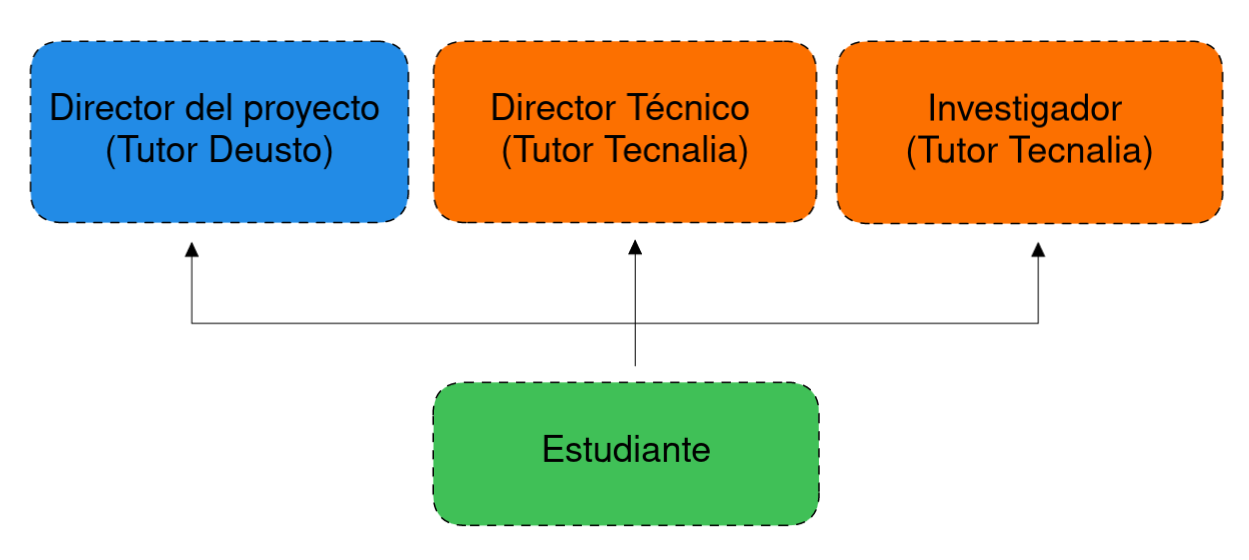
\includegraphics[width=\textwidth]{human-resources.png}
    \caption{Diagrama de recursos humanos}\label{fig:human-resources}
\end{figure}

\begin{itemize}
    \item \textbf{Director del proyecto:} El director del proyecto es la figura
          encargada de supervisar y coordinar todas las actividades del proyecto. Su papel
          es fundamental para establecer una visión clara, comunicar los objetivos y metas,
          y gestionar los recursos adecuados para alcanzarlos. Su experiencia en gestión de
          proyectos, habilidades de liderazgo y capacidad para tomar decisiones son
          fundamentales para asegurar la dirección correcta y el cumplimiento de los plazos
          establecidos.
    \item \textbf{Director Técnico:} El Director Técnico desempeña un papel crucial
          en la implementación exitosa del proyecto al proporcionar soporte técnico y
          garantizar la calidad y el rendimiento del producto final. Su experiencia
          técnica en el área específica del proyecto y su conocimiento profundo de las
          herramientas y tecnologías pertinentes permiten tomar decisiones informadas
          y resolver problemas técnicos de manera eficiente. Además, lidera y coordina al
          equipo técnico, asegurando la correcta implementación de las soluciones propuestas.
    \item \textbf{Investigador:} El investigador supervisa y controla la calidad del
          proyecto, identificando y proponiendo mejoras durante el proceso de desarrollo. Su
          enfoque en el control de calidad asegura la entrega de un producto final de alto nivel.
    \item \textbf{Estudiante:} El estudiante es el encargado de llevar a cabo el proyecto,
          este constituye su TFG y asume la responsabilidad de llevar a cabo todas las fases del
          mismo. Su participación abarca desde la investigación inicial hasta la implementación
          y evaluación final del proyecto. Como investigador principal, realiza una investigación
          exhaustiva sobre el tema del proyecto, recopilando información relevante y analizando
          los enfoques existentes en el campo. Con base en esta investigación, define los objetivos
          del proyecto y establece una estrategia para alcanzarlos.
\end{itemize}

\subsection{Programa de trabajo}
La siguiente sección detallará el programa de trabajo seguido en el proyecto,
incluyendo las diferentes tareas realizadas con su duración planificada y real,
junto con el diagrama de Gantt del proyecto. Las tareas del proyecto se han
dividido en tres fases distintas. La primera fase incluye la formación
necesarias para llevar a cabo el proyecto, así como la investigación inicial y
la definición de los objetivos. La segunda fase incluye la implementación de
las diferentes partes del proyecto, mientras que la tercera fase incluye la
experimentación, el análisis de resultados y la documentación final.

\subsubsection{Fase 1: Formación e investigación}
Esta fase está formada por una serie de tareas que se deben completar antes de
comenzar la implementación del proyecto. Las tareas incluidas en esta fase son
las siguientes:

\begin{itemize}
    \item \textbf{Tarea 1.1: Fundamentos de RL (1.5 semanas).} El objetivo de esta tarea es
          familiarizarse con los fundamentos del RL\@. Para ello, se realizará una investigación
          inicial sobre el tema, así como una serie de prácticas para familiarizarse con los
          conceptos básicos. La investigación inicial incluye la lectura de los capítulos 1, 3 y 6
          del libro \textit{Reinforcement Learning: An Introduction}\cite{sutton2018reinforcement}.
          Las prácticas incluyen la implementación de un notebook sobre Q-learning.
    \item \textbf{Tarea 1.2: Redes neuronales (1 semana).} El objetivo de esta tarea es
          investigar sobre las redes neuronales y familiarizarse con su funcionamiento. Para ello,
          se realizará una serie de prácticas sobre su funcionamiento e implementación.
    \item \textbf{Tarea 1.3: Algoritmos on-policy de RL (1 semana).} El objetivo de esta tarea
          es familiarizarse con los algoritmos de RL de tipo \textit{on-policy}.
    \item \textbf{Tarea 1.4: Stables-baselines (0.5 semanas).} Ejecutar ejemplos sencillos
          de la librería de RL \textit{Stables-baselines}\cite{stable-baselines3}.
    \item \textbf{Tarea 1.5: Introducción al FJSP y modelización (2.5 semanas).} El
          objetivo de esta tarea es comprender el problema del FJSP y proponer ideas de cómo
          modelizar el environment para poder aplicar RL\@.
    \item \textbf{Tarea 1.6: Conocer Imitation Learning (1 semana).} Por último, el objetivo
          de esta tarea es investigar sobre Imitation Learning y cómo aplicarlo al problema del
          FJSP\@.
\end{itemize}

\subsubsection{Fase 2: Implementación}
Esta fase está formada por una serie de tareas que incluyen la implementación
de las diferentes partes del proyecto. Las tareas incluidas en esta fase son
las siguientes:

\begin{itemize}
    \item \textbf{Tarea 2.1: Construcción pipeline básico (2 semanas).} El objetivo de esta tarea es combinar
          diferentes técnicas y algoritmos para crear un pipeline que provea de ejemplos a un modelo de
          Deep Learning mediante IL que sea capaz de aprender de planificaciones óptimas. Esta tarea básica busca
          una base sobre la que iterar y mejorar el proyecto en las siguientes tareas. Aquí se incluye la
          implementación básica del environment, la generación de instancias y la resolución de las mismas.
    \item \textbf{Tarea 2.2: Identificación del estado del proyecto (1 semana).} El objetivo de esta tarea es
          identificar los puntos fuertes y débiles del pipeline creado en la tarea anterior, así como
          las posibles mejoras que se pueden aplicar. A partir de aquí, se definirán las tareas
          necesarias para mejorar el pipeline.
    \item \textbf{Tarea 2.3: Implementación de redes neuronales de grafos en el environment (2 semanas).} El
          objetivo de esta tarea es refactorizar el environment para que la información de las operaciones
          y las máquinas se almacene en redes de grafos.
    \item \textbf{Tarea 2.4: Adaptación del agente al nuevo environment (1 semana).} Para esta tarea,
          se adaptará el agente de RL al nuevo environment creado en la tarea anterior. También se
          investigaran diferentes arquitecturas para el agente.
\end{itemize}

\subsubsection{Fase 3: Experimentación, análisis de resultados y documentación}
El último bloque de tareas incluye la experimentación, el análisis de los
resultados obtenidos y la documentación final del proyecto. Esta ultima es
fundamental debido a que el proyecto se desarrolla en un entorno de
investigación y es necesario documentar todo el procedimiento para que puede
ser aplicado por otros investigadores. Las tareas incluidas en esta fase son
las siguientes:

\begin{itemize}
    \item \textbf{Tarea 3.1: Optimización de hiperparámetros (2 semana).} Mediante Optuna se optimizarán los
          hiperparámetros del pipeline y se utilizaran los resultados obtenidos para mejorar los resultados del
          modelo.
    \item \textbf{Tarea 3.2: Análisis de resultados y aplicación de mejoras (1 semana).} Durante esta tarea se
          analizarán los resultados obtenidos y se aplicarán las mejoras necesarias para mejorar el rendimiento del
          modelo. Además, se realizará una comparación con los resultados obtenidos por otros autores en el mismo
          problema pero utilizando otras técnicas. Por último, se realizará una proceso de recolección de información
          para la redacción de la memoria del proyecto.
    \item \textbf{Tarea 3.3: Redacción de la memoria (2 meses).} Por último, se redactará la memoria del proyecto,
          donde se explicará en detalle la metodología desarrollada y los resultados obtenidos.
\end{itemize}

\subsubsection{Diagrama de Gantt}
A continuación se muestra el diagrama de Gantt del proyecto, donde se puede
observar la planificación temporal de las diferentes tareas descritas
anteriormente. El proyecto al estar dividido en tres fases se ha utilizado el
color azul para representar la fase 1, el color verde para la fase 2 y el color
morado para la fase 3. Se ha respetado cuidadosamente el tiempo de cada tarea y
el proyecto no ha sufrido ningún retraso durante su desarrollo.

\begin{figure}
    \centering
    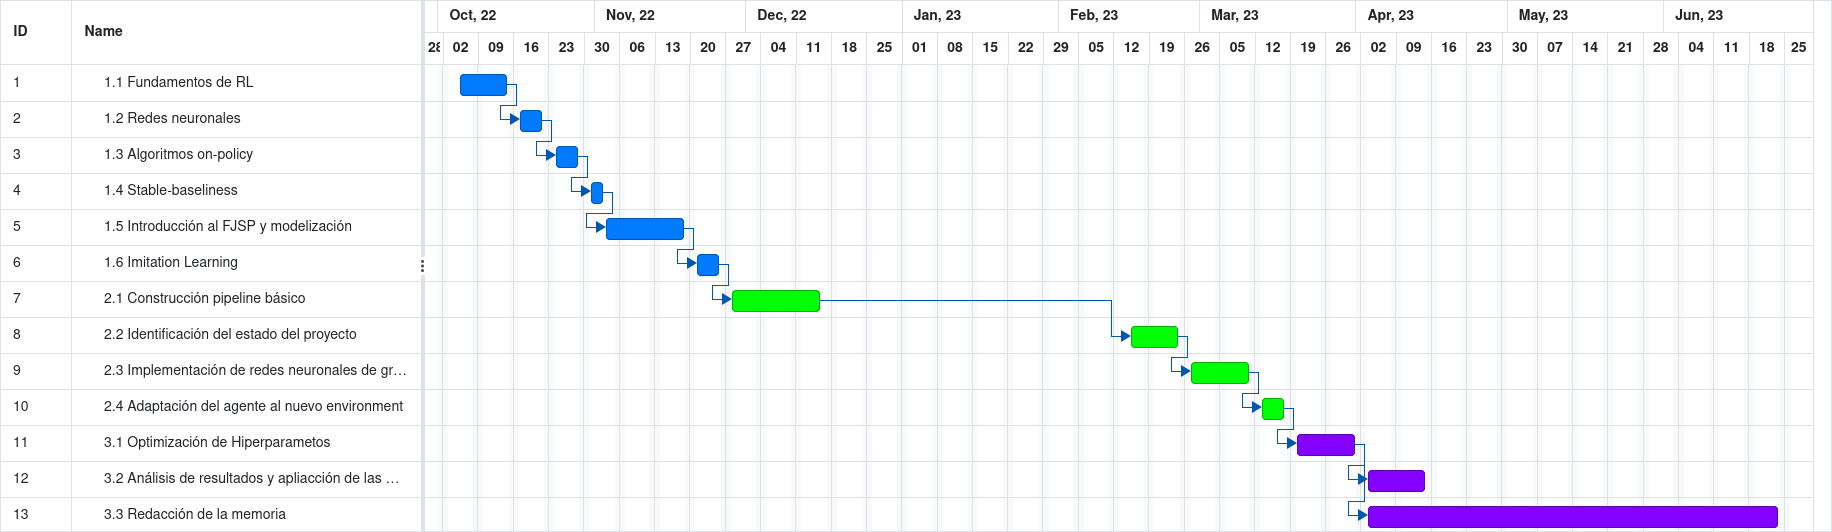
\includegraphics[angle=90, width=\textwidth, height=\textheight, keepaspectratio]{planificationgantt.png}
    \caption{Diagrama de planificación del proyecto.}\label{fig:gantt-planification}
\end{figure}

\subsection{Presupuesto}
La siguiente sección detallará el presupuesto necesario para llevar a cabo el
proyecto, incluyendo los diferentes recursos necesarios y su coste. El
presupuesto se ha dividido en tres categorías principales: recursos humanos,
hardware y software.

\subsubsection{Recursos humanos}
La siguiente tabla muestra el coste de los diferentes perfiles involucrados en
el proyecto, así como el número de horas invertidas por cada uno de ellos y el
coste total de cada perfil.

\begin{table}[ht]
    \centering
    \begin{tabular}[ht]{l|c|c|c}
        \textbf{Perfil}       & \textbf{Coste/Hora} & \textbf{Horas Invertidas} & \textbf{Precio Total} \\
        \hline
        Director del proyecto & 40\euro             & 20h                       & 800\euro              \\
        Director Técnico      & 90\euro             & 40h                       & 3.600\euro            \\
        Investigador          & 90\euro             & 40h                       & 3.600\euro            \\
        Estudiante            & 20\euro             & 300h                      & 6.000\euro            \\
    \end{tabular}
    \caption{Presupuesto de recursos humanos}\label{tab:huma-resources}
\end{table}

\subsubsection{Hardware}
La siguiente tabla muestra el coste de los diferentes recursos hardware
necesarios para llevar a cabo el proyecto, así como el número de unidades
necesarias y el coste total de cada recurso.

\begin{table}[ht]
    \centering
    \begin{tabular}[ht]{l|c|c|c}
        \textbf{Recurso}     & \textbf{Coste por unidad} & \textbf{Unidades} & \textbf{Precio Total} \\
        \hline
        Hora máquina virtual & 0.2\euro                  & 200u              & 40\euro               \\
        Portátil             & 700\euro                  & 1u                & 700\euro              \\
    \end{tabular}
    \caption{Presupuesto hardware}
    \label{tab:hardware-budget}
\end{table}

\subsubsection{Software}
Los recursos software necesarios para llevar a cabo el proyecto son gratuitos
en su mayoría, a excepción de la licencia de GitHub Copilot que tiene un coste
de 10\euro/mes. Aun así, se ha utilizado la versión gratuita que viene incluida
con la licencia de GitHub Pro por ser estudiante.

\subsubsection{Total}
\begin{table}
    \centering
    \begin{tabular}[ht]{l|r}
        \textbf{Recurso} & \textbf{Precio Total} \\
        \hline
        Recursos humanos & 14.000\euro           \\
        Hardware         & 740\euro              \\
        Software         & 0\euro                \\
        \hline
        Total            & 14.740\euro           \\
    \end{tabular}
    \caption{Presupuesto general}
    \label{tab:total-budget}
\end{table}

\pagebreak